\paragraph{base\_sum}

BaseSumGate is used to constrain the input to be composed of limbs which are arranged in little-endian. There are two kinds of constraints:

For each limb, limb is in range $[0, \text{base})$:
\[ \sum_{i=0}^{\text{base}}(\text{limb}_i - i) = 0. \]

Input is composed of limbs:
\[ \text{input} = \sum_{i=0}^{n-1} \text{limb}_{n-1-i} \times \text{base}^i. \]

The structure of gate is shown in \figref{fig:base-sum}.
\begin{figure}[!ht]
    \centering
    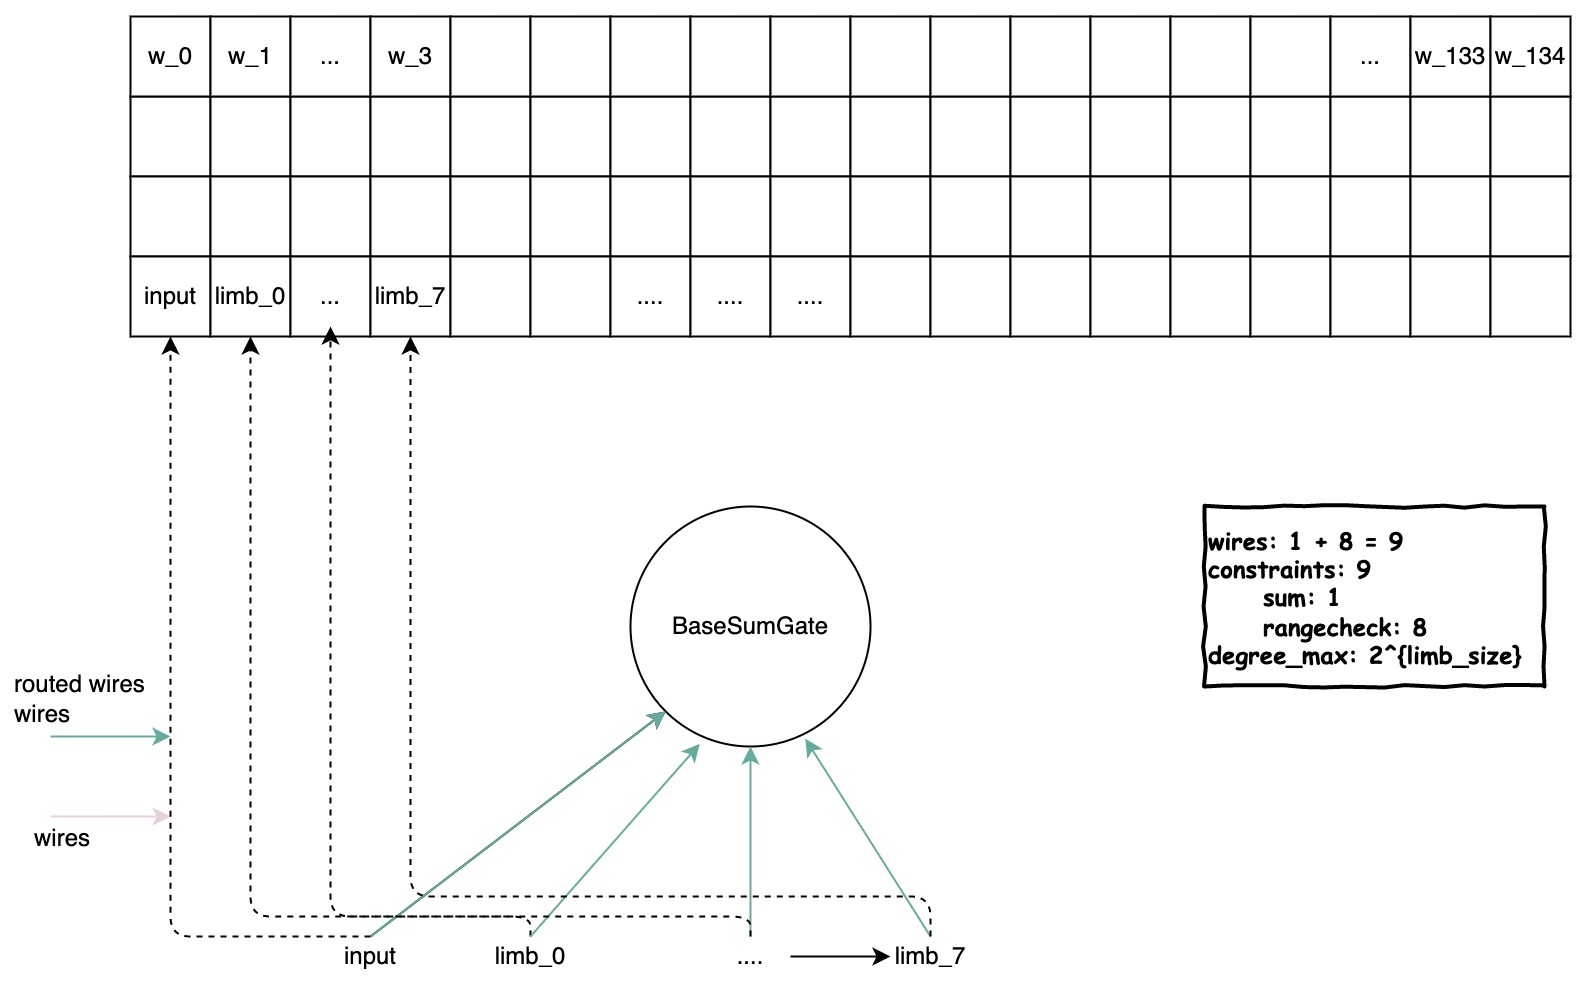
\includegraphics[width=0.6\textwidth]{gates/base_sum.jpeg}
    \caption{BaseSumGate}
    \label{fig:base-sum}
\end{figure}

There's 1 constraint for sum check and 8 constraints for limbs' range check. Degree of the gate is $2^{\text{limb\_size}}$ happens when limbs' range check.
